\documentclass[titlepage]{article}
\usepackage{graphicx}  % 插入图片
\usepackage{amsmath}  % 输入公式
\usepackage{bm}  % 加粗数学符号
\usepackage{listings}  % 插入代码
\usepackage{xcolor}  % 高亮代码

% 设置A4纸
\usepackage[a4paper]{geometry} 

\lstset{numbers=left, %设置行号位置
        numberstyle=\tiny, %设置行号大小
        keywordstyle=\color{blue}, %设置关键字颜色
        commentstyle=\color[cmyk]{1,0,1,0}, %设置注释颜色
        frame=single, %设置边框格式
        escapeinside=``, %逃逸字符(1左面的键),用于显示中文
        breaklines, %自动折行
        extendedchars=false, %解决代码跨页时,章节标题,页眉等汉字不显示的问题
        xleftmargin=2em,xrightmargin=2em, aboveskip=1em, %设置边距
        tabsize=4, %设置tab空格数
        showspaces=false %不显示空格
       }

% 文档信息
\title{\textbf{Advanced Control for Robotics: Homework \#1}}
\author{Shang Yangxing}
\date{\today}

\begin{document}

\maketitle

\section{ODE and Its Simulation}

\subsection{Equation of Pendulum Motions}

\begin{figure}[htbp]
    \centering
    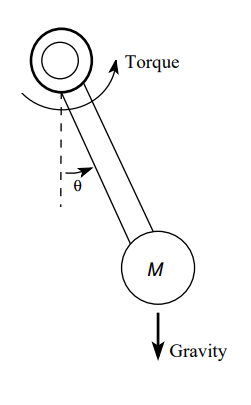
\includegraphics[width=.3\textwidth]{img/pendulum.png}
    \caption{pendulum model}
    \label{fig:pendulum}
\end{figure}

By applying the Newton's law of dynamics, a pendulum with no external force can be formulated as:

\begin{equation}
    ml^2 \ddot{\theta} + ml^2 \alpha \dot{\theta} + mgl \sin{\theta} - T = 0.
\end{equation}

in which,

\quad $m$ is mass of the ball

\quad $l$ is length of the rod

\quad $\alpha$ is the damping constant

\quad $g$ is the gravitational constant

\quad $\theta$ is angle measured between the rod and the vertical axis

\quad $T$ is torque of the joint, which is also the control input $u$

to a system of two first order equation by letting $x_1=\theta$, $x_2=\dot{\theta}$:

\begin{equation}
    \dot{x_1} = x_2, \quad \dot{x_2} = - \frac{g}{l}\sin{x_1} -\alpha x_2 + \frac{T}{ml^2}.
\end{equation}

Written in standard state-space form:

\begin{equation}
    \bm{\dot{x}} = 
    \begin{bmatrix}
        \dot{x_1} \\ \dot{x_2}
    \end{bmatrix}
    =
    \begin{bmatrix}
        x_2 \\ -\frac{g}{l}\sin{x_1} - \alpha x_2
    \end{bmatrix}
    +
    \begin{bmatrix}
        0 \\ \frac{1}{ml^2}
    \end{bmatrix}
    T
    \label{equ:state-space}
\end{equation}

\begin{equation}
    \bm{y} = 
    \begin{bmatrix}
        x_1 \\ x_2
    \end{bmatrix}
    = \bm{x}
\end{equation}

\subsection{Simulation of Pendulum}

When assuming $m=l=1$ with proper unit, equation (\ref{equ:state-space}) can be simplified as:

\begin{equation}
    \begin{bmatrix}
        \dot{x_1} \\ \dot{x_2}
    \end{bmatrix}
    =
    \begin{bmatrix}
        x_2 \\ -g\sin{x_1} - \alpha x_2 + T
    \end{bmatrix}
\end{equation}

according the equation, we code the simulation as following:

\lstinputlisting[language=Python]{1-2 simulation of pendulum.py}

and getting the output as:
\begin{figure}[htbp]
    \centering
    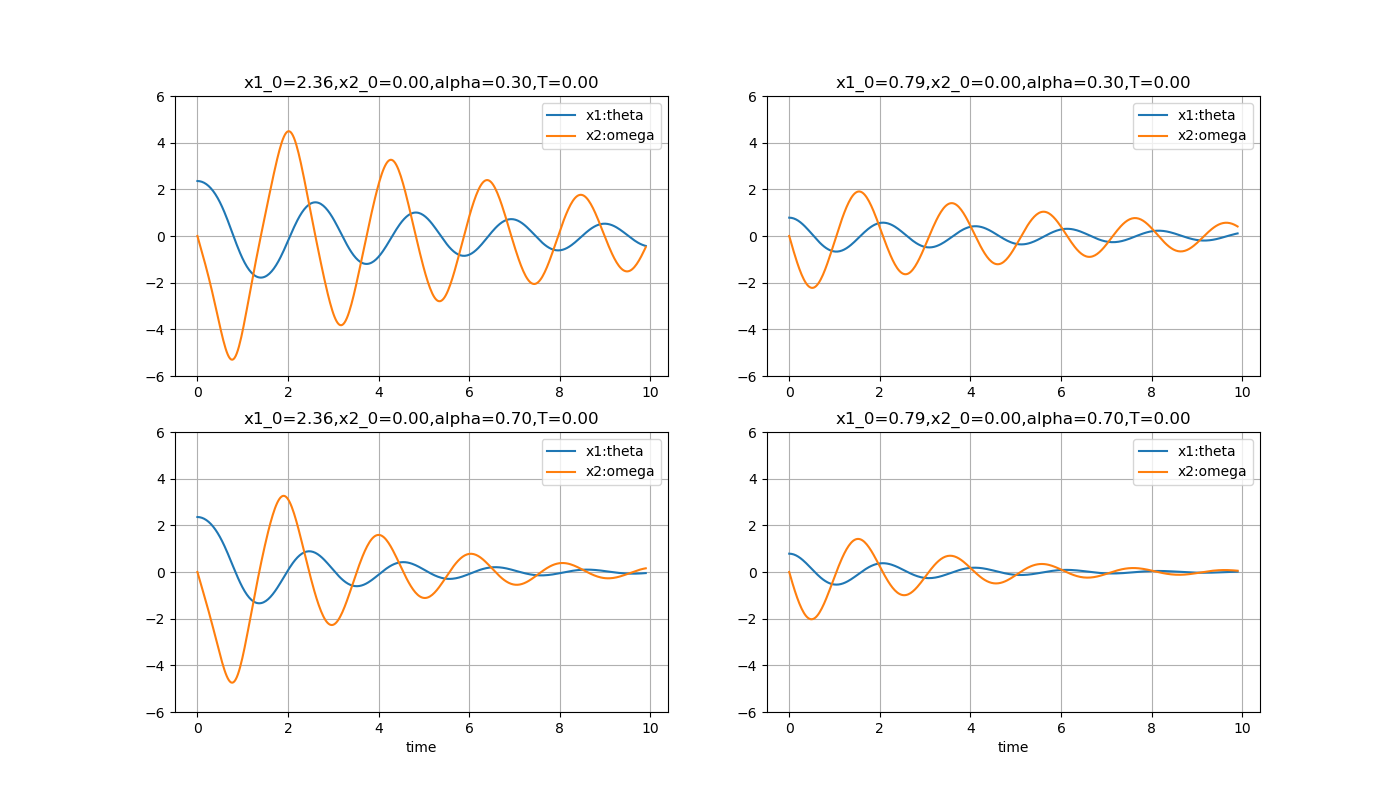
\includegraphics[width=\textwidth]{img/pendulumSim.png}
    \caption{pendulum simulation output}
    \label{fig:pendulumSim}
\end{figure}

\section{Matrix calculus}
\section{Inner product}
\section{Some linear algebra}
\section{Gradient Flow}

\end{document}